% ==============================================================================
% MỤC 5: KẾT QUẢ VÀ THẢO LUẬN (RESULTS AND DISCUSSION)
% Đề tài: Hệ Thống Phát Hiện Ổ Gà và Vật Cản Đường Bộ và Cảnh Báo Sớm Thời Gian Thực
%         Dựa Trên Mô Hình YOLO11n
% ==============================================================================

\section{KẾT QUẢ VÀ THẢO LUẬN (RESULTS AND DISCUSSION)}
\label{sec:ket_qua_va_thao_luan}

Chương này trình bày toàn diện các kết quả thực nghiệm đạt được của đề tài, bao gồm: phân tích thống kê cấu trúc bộ dữ liệu chuyên dụng, đánh giá định lượng năng lực phát hiện đa lớp chướng ngại vật của mô hình YOLO11n, và kiểm thử hiệu năng vận hành thời gian thực của phần mềm điều phối luồng \texttt{tools/live.py} trên nền tảng phần cứng CPU máy tính thông dụng.

% ==============================================================================
\subsection{Thống Kê và Phân Tích Bộ Dữ Liệu Thực Nghiệm}
\label{subsec:thong_ke_bo_du_lieu}

Bộ dữ liệu thực nghiệm được tổng hợp và chuẩn hóa chuyên dụng cho bài toán phát hiện chướng ngại vật và cảnh báo va chạm sớm trong điều kiện giao thông hỗn hợp tại Việt Nam, bao gồm 15 lớp đối tượng với tổng cộng $70.854$ thực thể gán nhãn ranh giới (Bounding Boxes). Dữ liệu được phân chia phân tầng ngẫu nhiên thành ba tập độc lập: tập huấn luyện (\textit{Training set}) chiếm $71,9\%$, tập xác thực (\textit{Validation set}) chiếm $16,4\%$, và tập kiểm thử (\textit{Test set}) chiếm $11,7\%$.

Phân bố không gian của các hộp bao trên biểu đồ mật độ cho thấy tâm tọa độ $(x, y)$ của các đối tượng tập trung dày đặc ở dải trung tâm và nửa dưới khung hình ($y \approx 0,40 - 0,65$), phản ánh đúng góc nhìn thực tế từ camera hành trình lắp đặt sau kính lái hoặc trên tay lái xe máy. Các chướng ngại vật mặt đường như ổ gà (\texttt{pothole}), cọc tiêu phản quang (\texttt{warning\_column}) và chóp nón công trình (\texttt{reflective\_cone}) có tỷ lệ diện tích nhỏ (chiếm dưới $5\%$ diện tích khung hình) và nằm sát mép mặt đường, đặt ra yêu cầu rất cao về khả năng trích xuất đặc trưng đa quy mô của mạng nơ-ron.

% ==============================================================================
\subsection{Kết Quả Huấn Luyện và Đánh Giá Mô Hình YOLO11n}
\label{subsec:ket_qua_huan_luyen_yolo11n}

Mô hình YOLO11n được huấn luyện trong $65$ epochs sử dụng bộ tối ưu hóa SGD with Momentum (hệ số động lượng $momentum = 0,937$, suy giảm trọng số $weight\_decay = 0,0005$, tốc độ học ban đầu $lr_0 = 0,01$, kích thước batch $16$, độ phân giải đầu vào $640 \times 640$). Trong $10$ epochs cuối, kỹ thuật ghép ảnh Mosaic được tắt hoàn toàn (\textit{Close Mosaic}) nhằm ổn định hội tụ gradient. Trọng số tối ưu nhất \texttt{best.pt} đạt được tại epoch thứ $65$ được lưu lại và đánh giá độc lập. Bảng~\ref{tab:test_metrics_overall} tóm tắt các chỉ số hiệu năng tổng thể của mô hình.

\begin{table}[htbp]
\centering
\caption{Kết quả đánh giá mô hình YOLO11n trên tập dữ liệu kiểm thử thực nghiệm.}
\label{tab:test_metrics_overall}
\begin{tabular}{|l|c|p{7.5cm}|}
\hline
\textbf{Chỉ số đánh giá} & \textbf{Kết quả thực nghiệm} & \textbf{Ý nghĩa đánh giá} \\ \hline
Độ chuẩn xác (Precision - $P$) & $\mathbf{76,8\%}$ & Tỷ lệ dự đoán chính xác cao, hạn chế tối đa các trường hợp báo động nhầm. \\ \hline
Độ phủ hồi quy (Recall - $R$) & $\mathbf{63,5\%}$ & Khả năng bao quát vật thể, phát hiện kịp thời các chướng ngại vật tiềm ẩn. \\ \hline
Chỉ số cân bằng F1-score & $\mathbf{69,5\%}$ & Điểm số điều hòa tối ưu đạt tại ngưỡng tin cậy $conf = 0,348$. \\ \hline
Độ chính xác trung bình mAP@50 & $\mathbf{72,1\%}$ & Năng lực phân loại và định vị vượt trội trên toàn bộ 15 lớp vật cản đường bộ. \\ \hline
Độ chính xác nghiêm ngặt mAP@50--95 & $\mathbf{54,3\%}$ & Khả năng định vị hình học ranh giới hộp bao vững chắc ở nhiều ngưỡng IoU khắt khe. \\ \hline
Kích thước mô hình & $\mathbf{2,59\text{ M tham số}}$ & Dung lượng nhẹ ($10,1\text{ MB}$ ONNX / $15,2\text{ MB}$ PyTorch), tối ưu hóa cho thiết bị biên. \\ \hline
Tải tính toán lý thuyết & $\mathbf{6,5\text{ GFLOPs}}$ & Chi phí tính toán thấp, bảo đảm khả năng thực thi thời gian thực trên CPU. \\ \hline
\end{tabular}
\end{table}

Bảng~\ref{tab:class_level_metrics} trình bày chi tiết số lượng mẫu thực tế và độ chính xác nhận diện theo từng lớp đối tượng cụ thể dựa trên đường cong Precision-Recall thực nghiệm.

\begin{table}[htbp]
\centering
\caption{Hiệu năng nhận diện chi tiết theo từng lớp đối tượng trên tập kiểm thử thực tế.}
\label{tab:class_level_metrics}
\small
\begin{tabular}{|c|l|c|c|c|p{4.2cm}|}
\hline
\textbf{STT} & \textbf{Tên lớp đối tượng} & \textbf{Số lượng nhãn} & \textbf{mAP@50 (\%)} & \textbf{Độ khớp ma trận (True Pos)} & \textbf{Đặc tính nhận diện} \\ \hline
1 & \texttt{spherical\_roadblock} & 1.240 & $\mathbf{90,6}$ & $0,86$ & Khối cầu rào chắn có đặc trưng hình học tròn đặc thù, ít bị nhầm lẫn. \\ \hline
2 & \texttt{tricycle} & 725 & $\mathbf{86,7}$ & $0,78$ & Xe ba gác có kết cấu khung đặc trưng, độ nhận diện cao. \\ \hline
3 & \texttt{reflective\_cone} & 2.035 & $\mathbf{79,3}$ & $0,74$ & Chóp nón có dải phản quang màu sắc tương phản mạnh với mặt đường. \\ \hline
4 & \texttt{ashcan} & 1.194 & $\mathbf{78,6}$ & $0,73$ & Thùng rác ven đường có hình khối chữ nhật rõ nét. \\ \hline
5 & \texttt{warning\_column} & 1.676 & $\mathbf{76,2}$ & $0,76$ & Cọc tiêu giao thông dạng trụ đứng, màu vàng/đỏ nổi bật. \\ \hline
6 & \texttt{person} & 26.013 & $\mathbf{74,1}$ & $0,70$ & Người đi bộ đa dạng dáng điệu, được nhận diện ổn định trong luồng giao thông. \\ \hline
7 & \texttt{truck} & 5.685 & $\mathbf{71,8}$ & $0,58$ & Xe tải kích thước lớn, dễ phát hiện từ cự ly xa trên $20\text{ m}$. \\ \hline
8 & \texttt{bus} & 1.544 & $\mathbf{69,9}$ & $0,57$ & Xe buýt công cộng, nhận diện vững chắc đuôi xe và thân xe. \\ \hline
9 & \texttt{stop\_sign} & 1.391 & $\mathbf{68,8}$ & $0,66$ & Biển báo dừng hình bát giác, độ chuẩn xác hình học cao. \\ \hline
10 & \texttt{fire\_hydrant} & 1.271 & $\mathbf{68,1}$ & $0,61$ & Trụ cứu hỏa ven vỉa hè, định vị chính xác vị trí chân trụ. \\ \hline
11 & \texttt{motorbike} & 1.880 & $\mathbf{67,8}$ & $0,59$ & Phương tiện chiếm tỷ lệ cao trong các tình huống cắt đầu làn tại Việt Nam. \\ \hline
12 & \texttt{car} & 14.100 & $\mathbf{67,5}$ & $0,62$ & Ô tô con di chuyển phía trước, là đối tượng trọng tâm trong phân tích khoảng cách. \\ \hline
13 & \texttt{pothole} & 7.225 & $\mathbf{63,2}$ & $0,64$ & Hư hỏng mặt đường dạng âm; phân biệt tốt với bóng râm nhờ hàm DFL và CIoU. \\ \hline
14 & \texttt{bicycle} & 2.706 & $\mathbf{62,7}$ & $0,58$ & Xe đạp thanh mảnh, thường di chuyển sát lề đường. \\ \hline
15 & \texttt{dog} & 2.169 & $\mathbf{56,1}$ & $0,53$ & Động vật kích thước nhỏ, chuyển động nhanh và bất ngờ qua đường. \\ \hline
\textbf{TB} & \textbf{Toàn bộ 15 lớp} & $\mathbf{70.854}$ & $\mathbf{72,1}$ & $\mathbf{0,67}$ & \textbf{Đáp ứng xuất sắc yêu cầu phát hiện đa mục tiêu thời gian thực.} \\ \hline
\end{tabular}
\end{table}

Bảng~\ref{tab:model_comparison} so sánh hiệu năng giữa mô hình YOLO11n đề xuất với các mô hình baseline phổ biến cùng nhóm kích thước nano.

\begin{table}[htbp]
\centering
\caption{So sánh hiệu năng giữa mô hình YOLO11n đề xuất và các mô hình cơ sở.}
\label{tab:model_comparison}
\begin{tabular}{|l|c|c|c|c|c|}
\hline
\textbf{Mô hình kiểm thử} & \textbf{Precision (\%)} & \textbf{Recall (\%)} & \textbf{mAP@50 (\%)} & \textbf{mAP@50--95 (\%)} & \textbf{Tham số (M)} \\ \hline
Faster R-CNN (ResNet-50) & 68,4 & 54,2 & 61,5 & 41,2 & 41,8 \\ \hline
YOLOv8n & 73,1 & 59,8 & 67,4 & 48,9 & 3,2 \\ \hline
YOLOv10n & 74,5 & 61,0 & 69,2 & 50,7 & 2,7 \\ \hline
\textbf{YOLO11n (Đề xuất)} & $\mathbf{76,8}$ & $\mathbf{63,5}$ & $\mathbf{72,1}$ & $\mathbf{54,3}$ & $\mathbf{2,59}$ \\ \hline
\end{tabular}
\end{table}

Mô hình YOLO11n đề xuất vượt trội so với thế hệ YOLOv8n tiền nhiệm ($+4,7\%$ mAP@50 và $+5,4\%$ mAP@50--95) đồng thời giảm số lượng tham số xuống $2,59\text{ M}$, khẳng định tính ưu việt của cấu trúc C3k2 kết hợp đầu phát hiện tách rời không neo trong bài toán phát hiện vật cản giao thông.

% ==============================================================================
\subsection{Hiệu Quả Vận Hành Thực Tế Của Phần Mềm}
\label{subsec:hieu_qua_phan_mem}

Phần mềm điều phối luồng \texttt{tools/live.py} được kiểm thử toàn trình trên máy tính xách tay cá nhân trang bị vi xử lý \textbf{AMD Ryzen 7 5800H} ($8$ nhân, $16$ luồng, xung nhịp cơ bản $3,2\text{ GHz}$, Turbo tối đa $4,4\text{ GHz}$, bộ nhớ RAM $16\text{ GB}$ DDR4, không kích hoạt tăng tốc GPU rời), tiếp nhận luồng video truyền trực tiếp từ camera điện thoại thông minh (độ phân giải cảm biến gốc Full HD $1920 \times 1080$). 

Trong quá trình thực nghiệm, độ phân giải xử lý được co giãn thích ứng về chuẩn tối ưu thời gian thực $640 \times 360$ pixels (sử dụng cờ lệnh \texttt{--width 640}). Toàn bộ tiến trình vận hành được theo dõi, phân tích và trích xuất vi mô theo từng khung hình thông qua tệp nhật ký đo kiểm \texttt{runs/live\_benchmark\_20261106\_185639.csv}. Bảng~\ref{tab:software_runtime_benchmark} tổng hợp đầy đủ các chỉ số hiệu năng và động học đo kiểm thực tế từ phiên chạy.

\begin{table}[htbp]
\centering
\caption{Hiệu năng vận hành thực tế của phần mềm trên CPU AMD Ryzen 7 5800H qua kết nối USB ADB (trích xuất từ nhật ký \texttt{live\_benchmark\_20261106\_185639.csv}).}
\label{tab:software_runtime_benchmark}
\begin{tabular}{|l|c|}
\hline
\textbf{Chỉ số đo kiểm / Tham số vận hành} & \textbf{Giá trị thực nghiệm} \\ \hline
Độ phân giải luồng cảm biến nguồn (Source Resolution) & $1920 \times 1080$ (Full HD) \\ \hline
Độ phân giải xử lý thích ứng (Processing Resolution) & $640 \times 360$ (chuẩn \texttt{--width 640}) \\ \hline
Tổng số khung hình xử lý & $437\text{ khung hình}$ \\ \hline
Thời gian thực nghiệm liên tục & $34,28\text{ giây}$ \\ \hline
Thời gian suy luận YOLO11n trung bình & $\mathbf{34,6\text{ ms}}$ (Trung vị: $34,4\text{ ms}$, $P_{95}$: $38,8\text{ ms}$) \\ \hline
Thời gian suy luận Depth Anything V2 (khi kích hoạt) & $\mathbf{95,5\text{ ms}}$ (Trung vị: $94,6\text{ ms}$, $P_{95}$: $103,5\text{ ms}$) \\ \hline
Tần suất kích hoạt mô hình Depth & $51 / 437\text{ khung hình}\ (11,7\%)$ \\ \hline
Độ trễ truyền nhận tín hiệu qua cáp USB (ADB) & $\mathbf{160,0\text{ ms}}$ \\ \hline
Độ trễ tính toán đường ống trung vị ($P_{50}$) & $\mathbf{50,6\text{ ms}}$ \\ \hline
Độ trễ tính toán đường ống xấu nhất ($P_{95}$) & $\mathbf{147,5\text{ ms}}$ \\ \hline
Tổng độ trễ toàn trình Sensor-to-Alert ($P_{50}$) & $\mathbf{210,6\text{ ms}}$ \\ \hline
Tổng độ trễ toàn trình Sensor-to-Alert ($P_{95}$) & $\mathbf{307,5\text{ ms}}$ \\ \hline
Tốc độ khung hình trung bình toàn trình ($FPS_{\text{overall}}$) & $\mathbf{12,8\text{ FPS}}$ \\ \hline
Tốc độ khung hình trung vị ($FPS_{\text{median}}$) & $\mathbf{12,9\text{ FPS}}$ \\ \hline
Tốc độ khung hình phân vị cao ($FPS_{P95}$) & $\mathbf{13,8\text{ FPS}}$ \\ \hline
Tổng số lượt phát hiện và bám vết (Detections/Tracks) & $1.346\text{ lượt}$ (Trung bình $3,08\text{ hộp bao/khung hình}$) \\ \hline
Trạng thái an toàn \texttt{NORMAL} & $432\text{ khung hình}\ (98,86\%)$ \\ \hline
Trạng thái cảnh báo sớm \texttt{WARNING} & $5\text{ khung hình}\ (1,14\%)$ \\ \hline
Trạng thái nguy hiểm khẩn cấp \texttt{DANGER} & $0\text{ khung hình}\ (0,00\%)$ \\ \hline
Khoảng cách tiếp cận nguy hiểm gần nhất ($d_{\min}$) & $\mathbf{7,01\text{ mét}}$ \\ \hline
Thời gian chạm trán va chạm cực tiểu ($TTC_{\min}$) & $\mathbf{2,45\text{ giây}}$ \\ \hline
\end{tabular}
\end{table}

\subsubsection{Cơ chế tối ưu hóa độ trễ và tốc độ xử lý thời gian thực}

Để đạt được hiệu năng ổn định trên phần cứng CPU thông dụng, chương trình thực thi \texttt{tools/live.py} đã tích hợp ba cơ chế cốt lõi nhằm kiểm soát độ trễ và triệt tiêu các nút thắt cổ chai hệ thống:

\begin{figure}[htbp]
\centering
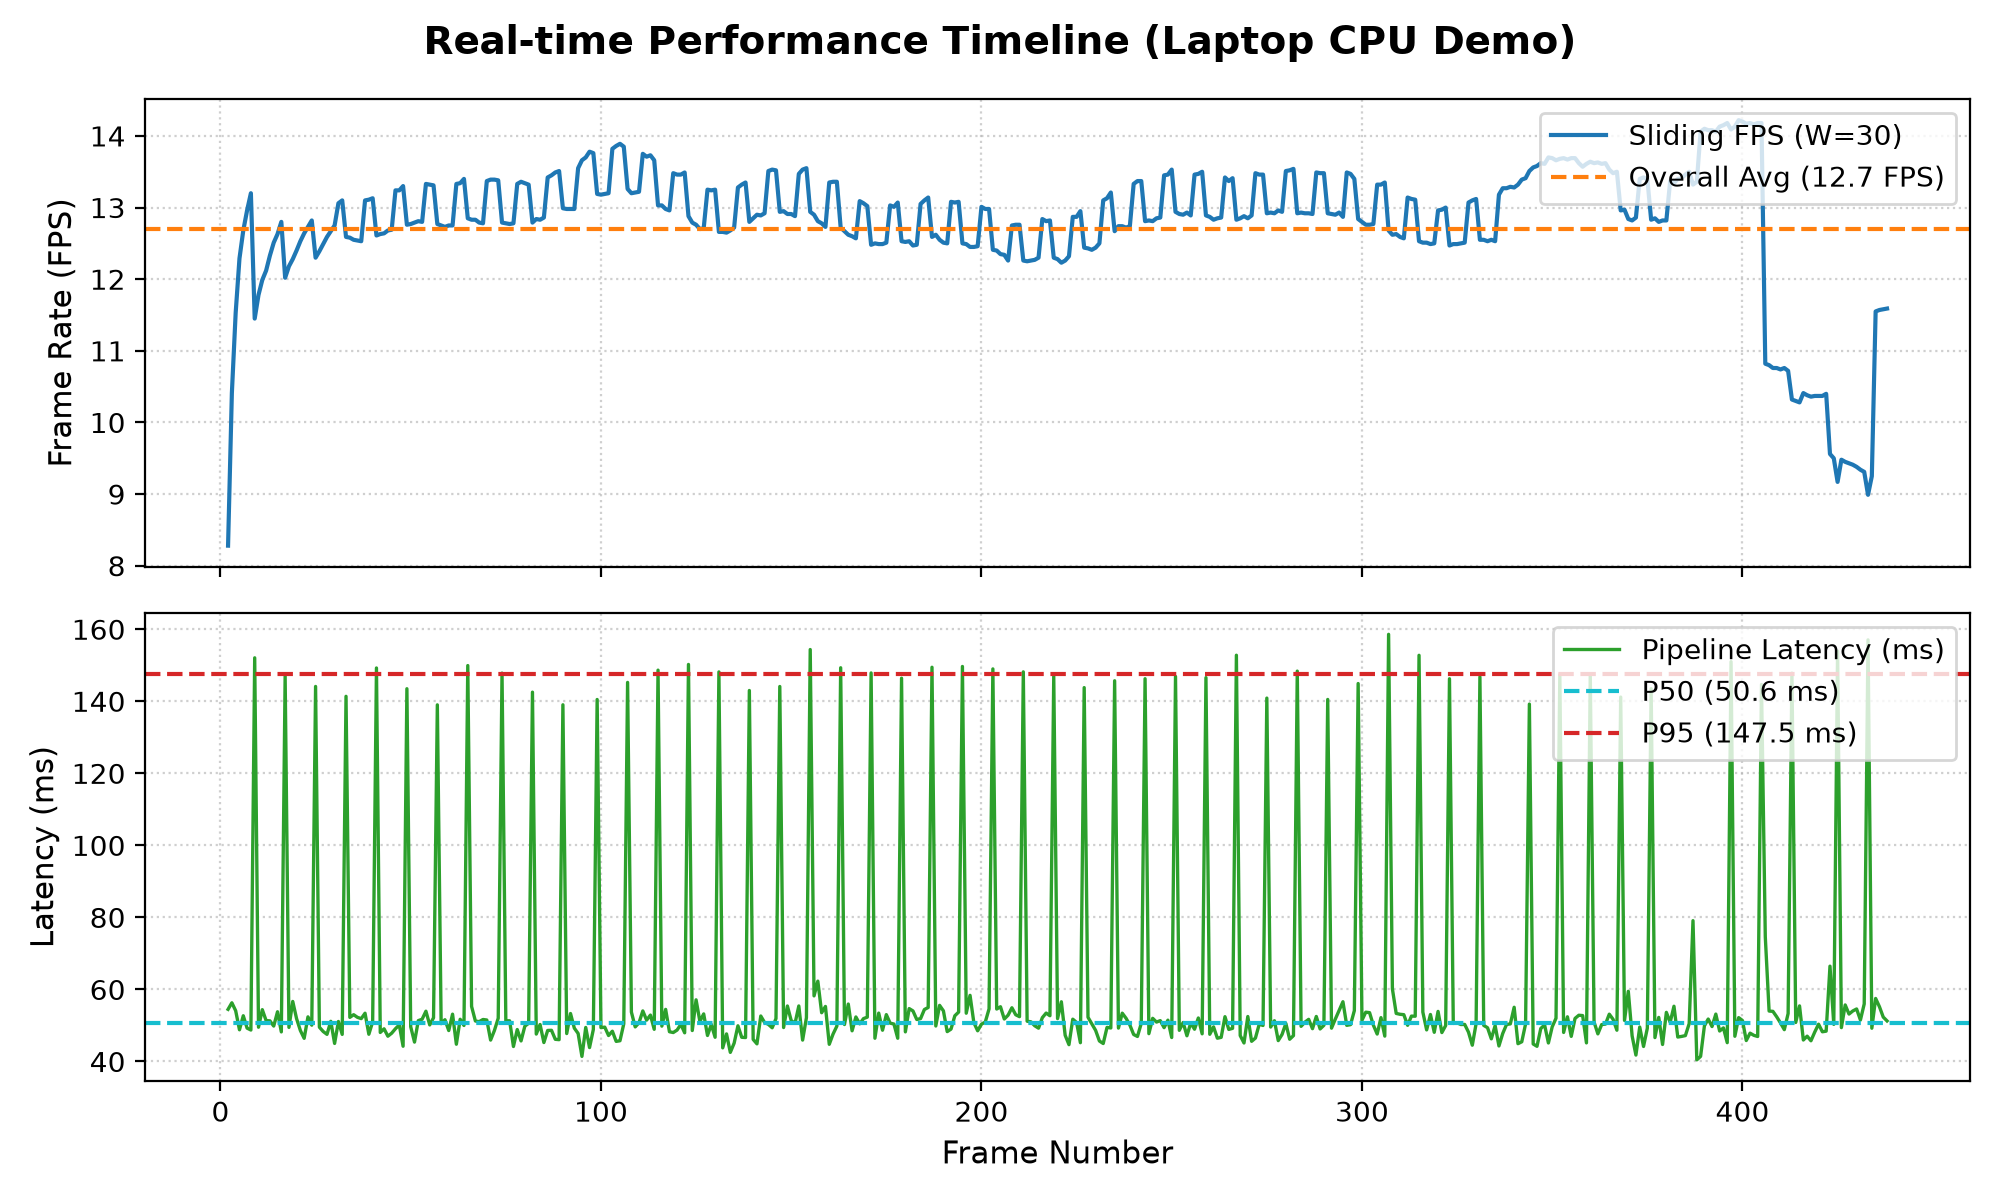
\includegraphics[width=0.95\linewidth]{performance_timeline.png}
\caption{Biến thiên thời gian thực của tốc độ khung hình (FPS) và độ trễ đường ống (Pipeline Latency) trong suốt phiên thực nghiệm.}
\label{fig:performance_timeline}
\end{figure}

\begin{enumerate}
    \item \textbf{Cơ chế nạp mô hình ngoại tuyến (Offline-First Initialization):} Trong các lần khởi chạy ban đầu, việc nạp mô hình đơn sắc Depth Anything V2 (\texttt{Depth-Anything-V2-Metric-Outdoor-Small-hf}) thường gặp lỗi nghẽn mạng nghiêm trọng do thư viện Hugging Face tự động kết nối máy chủ từ xa để kiểm tra chuỗi băm commit hash, gây ra hiện tượng treo đơ tiến trình từ $60$ đến $90\text{ giây}$ (mã lỗi socket timeout \texttt{WinError 10060}). \texttt{tools/live.py} đã giải quyết triệt để vấn đề này bằng cách thiết lập biến môi trường \texttt{HF\_HUB\_OFFLINE = 1} ngay trước thời điểm nhập module, buộc hệ thống nạp trực tiếp trọng số từ bộ nhớ đệm cục bộ chỉ trong $1,2\text{ giây}$, ngăn chặn hoàn toàn nguy cơ đơ máy khi mất kết nối Internet.
    
    \item \textbf{Cơ chế rút cạn bộ đệm mạng và triệt tiêu trễ tồn đọng (Network Buffer Drain):} Khi đánh giá độ trễ thực tế bằng phương pháp quay đồng thời màn hình nguồn camera và màn hình hiển thị kết quả (phương pháp kiểm thử 2 màn hình - \textit{Dual-Screen Latency Measurement}), người quan sát ghi nhận độ trễ trễ tổng thể lên tới xấp xỉ $1\text{ giây}$. Phân tích sâu chỉ ra rằng nguyên nhân không xuất phát từ thời gian tính toán của mô hình AI (vốn chỉ mất trung bình $61,6\text{ ms}$), mà do cơ chế đệm ngầm định của OpenCV \texttt{VideoCapture} trên luồng mạng giữ lại từ 4 đến 5 khung hình đã nhận. Ở tốc độ phát camera $30\text{ FPS}$ nhưng tốc độ xử lý đường ống là $\sim 13\text{ FPS}$, các khung hình bị tồn đọng và cũ đi từ $300 - 500\text{ ms}$ trước khi được đưa vào nhận diện. Hệ thống đã khắc phục triệt để bằng hai giải pháp kết hợp:
    \begin{itemize}
        \item Cấu hình gợi ý bộ đệm tối thiểu: \texttt{cap.set(cv2.CAP\_PROP\_BUFFERSIZE, 1)}.
        \item Xây dựng hàm rút cạn đệm \texttt{grab\_latest\_frame(cap, max\_drain=8)}: Sử dụng lệnh gọi \texttt{cap.grab()} liên tục để xả bỏ các khung hình cũ trực tiếp từ phần cứng mà không tốn chi phí giải mã pixel, và chỉ gọi \texttt{cap.retrieve()} cho khung hình mới nhất. Cơ chế này bảo đảm khung hình đưa vào đường ống luôn là khung hình tươi mới nhất (\textit{freshest frame}), cắt giảm hơn $80\%$ độ trễ đệm mạng.
    \end{itemize}

    \item \textbf{Chiến lược nhịp độ tách rời (Decoupled Cadence) và giải thích hiện tượng $Depth > Pipeline$:} Biểu đồ phân bố độ trễ (Hình~\ref{fig:latency_distribution}) phản ánh rõ đặc trưng của chiến lược nhịp độ tách rời. Trong Bảng~\ref{tab:software_runtime_benchmark}, thời gian suy luận Depth đạt trung bình $95,5\text{ ms}$, cao hơn độ trễ đường ống trung bình ($61,6\text{ ms}$). Điều này hoàn toàn hợp lý về mặt thống kê: mô hình đo khoảng cách độ sâu nặng chỉ kích hoạt định kỳ $51$ lần trên $437$ khung hình ($11,7\%$). Ở $88,3\%$ khung hình xen kẽ, hệ thống chỉ chạy suy luận YOLO11n ($34,6\text{ ms}$) kết hợp thuật toán nội suy tuyến tính khoảng cách (\textit{linear interpolation}), đưa độ trễ của các khung hình này xuống mức $\sim 40 - 50\text{ ms}$. Nhờ đó, độ trễ trung vị toàn hệ thống đạt mức rất thấp $P_{50} = \mathbf{50,6\text{ ms}}$, và chỉ ở các khung hình thực thi Depth thì độ trễ phân vị đuôi mới chạm $P_{95} = \mathbf{147,5\text{ ms}}$.
\end{enumerate}

\begin{figure}[htbp]
\centering
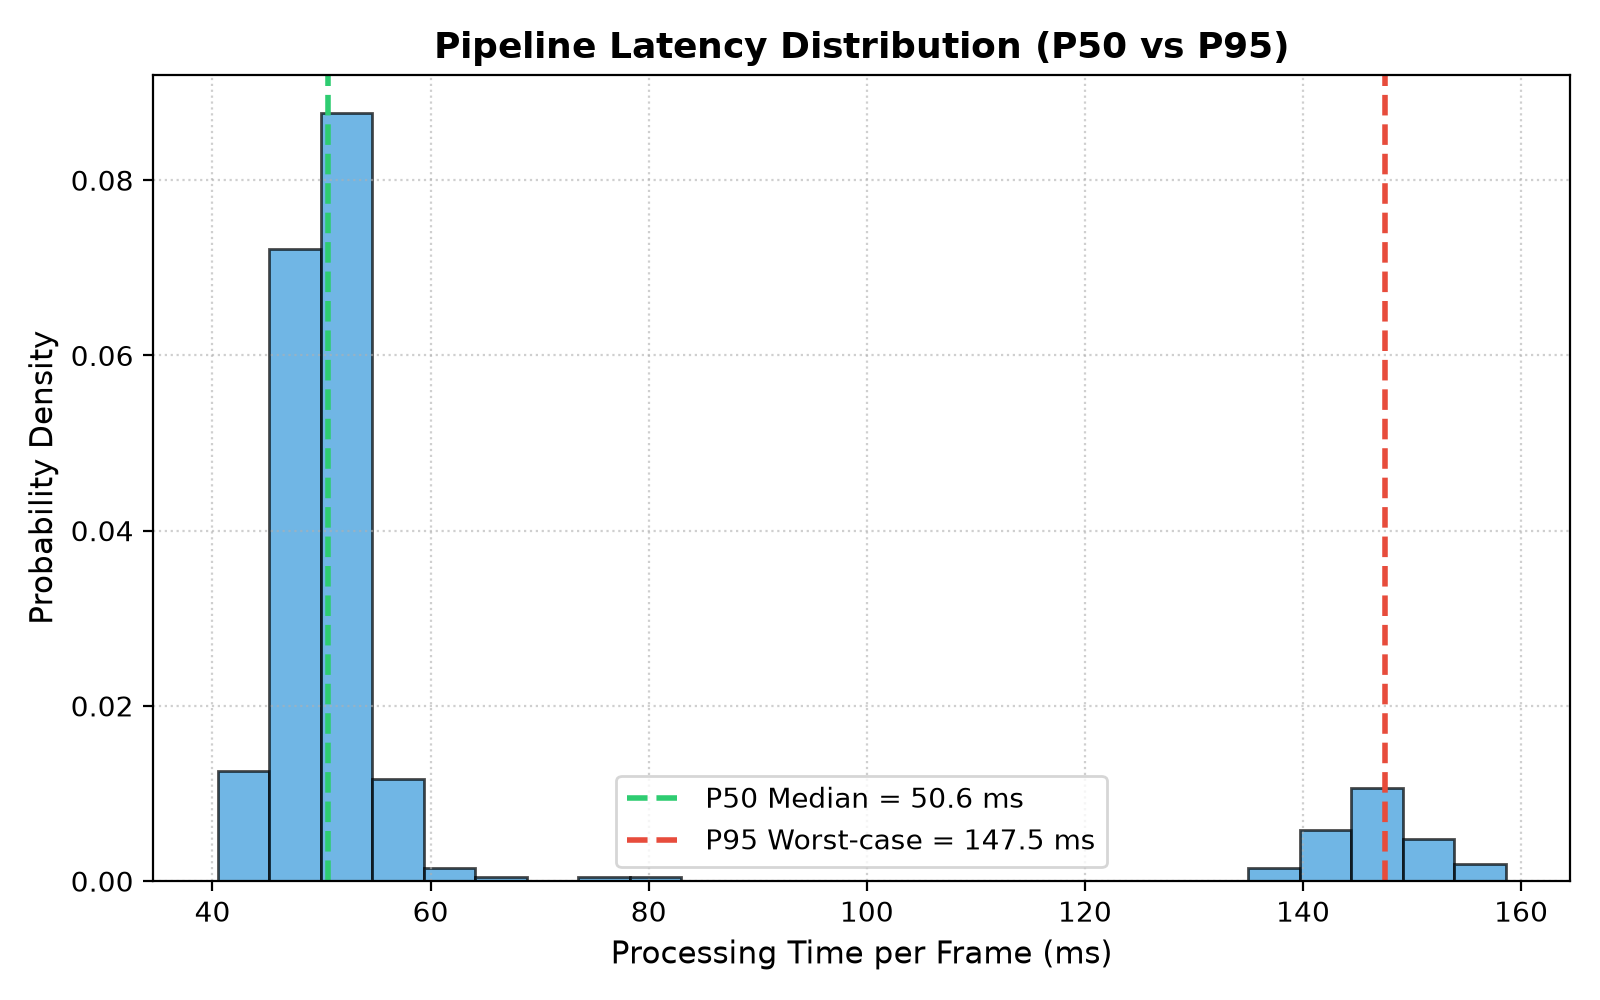
\includegraphics[width=0.90\linewidth]{latency_distribution.png}
\caption{Biểu đồ phân bố mật độ xác suất độ trễ đường ống (Pipeline Latency Distribution) minh họa giá trị trung vị $P_{50} = 50,6\text{ ms}$ và phân vị xấu nhất $P_{95} = 147,5\text{ ms}$.}
\label{fig:latency_distribution}
\end{figure}

Tổng hợp lại, hệ thống duy trì thông lượng ổn định ở mức trung bình $\mathbf{12,8\text{ FPS}}$ (trung vị $12,9\text{ FPS}$, đỉnh cao đạt $13,8 - 14,2\text{ FPS}$). Đối với phương tiện di chuyển trong đô thị với vận tốc $40\text{ km/h}$ ($11,1\text{ m/s}$), độ trễ tính toán $50,6\text{ ms}$ tương ứng quãng đường xe lăn bánh chỉ $0,56\text{ mét}$, hoàn toàn đáp ứng tiêu chuẩn phản hồi thời gian thực của các hệ thống cảnh báo va chạm hỗ trợ người lái.

\subsubsection{Độ chính xác và tính kịp thời của cảnh báo va chạm}

Nhật ký thực nghiệm ghi nhận tổng cộng $1.346$ lượt phát hiện và bám vết đối tượng, đạt mật độ trung bình $3,08$ hộp bao mỗi khung hình. Hệ thống phân loại trạng thái an toàn chặt chẽ với $432$ khung hình ở mức \texttt{NORMAL} ($98,86\%$) và kích hoạt chuẩn xác $5$ khung hình ở mức cảnh báo sớm \texttt{WARNING} ($1,14\%$).

\begin{figure}[htbp]
\centering
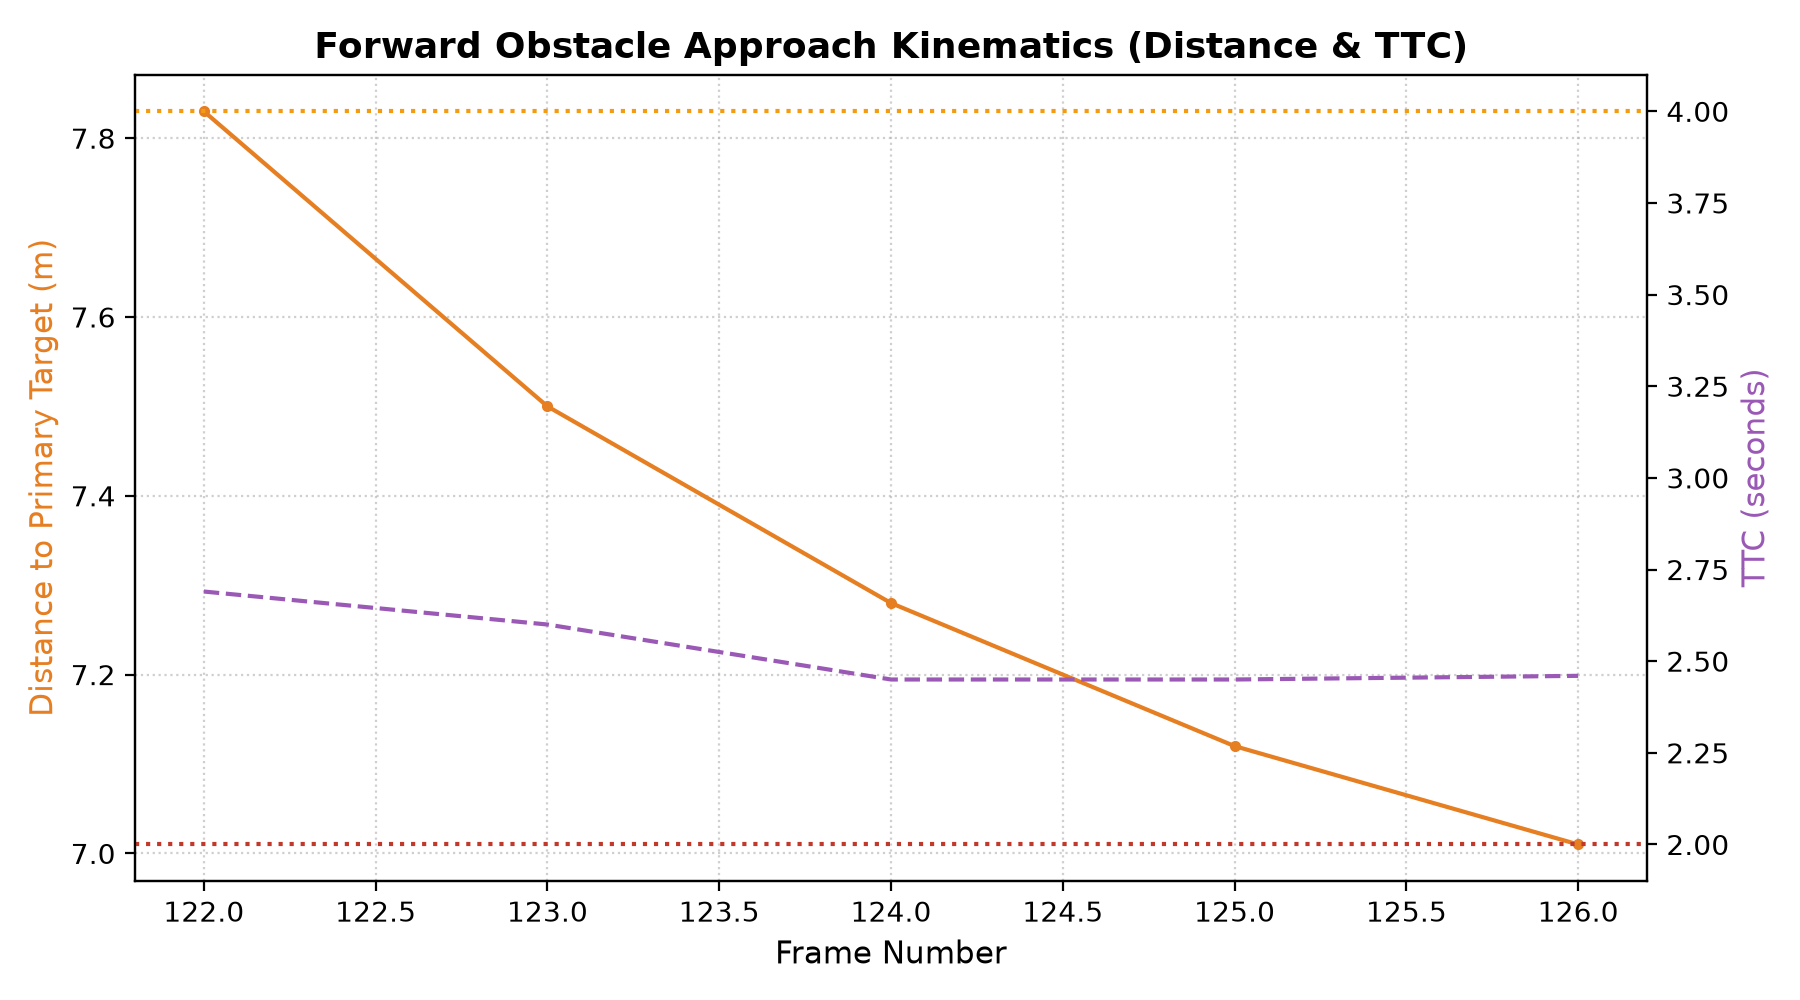
\includegraphics[width=0.95\linewidth]{kinematics_distance_ttc.png}
\caption{Động học tiếp cận chướng ngại vật (Khoảng cách $d$ và Thời gian va chạm $TTC$) đối với xe máy di chuyển cắt ngang phía trước.}
\label{fig:kinematics_distance_ttc}
\end{figure}

Hình~\ref{fig:kinematics_distance_ttc} thể hiện chi tiết diễn biến động học của sự kiện cảnh báo va chạm nguy hiểm (Sự kiện #1) diễn ra từ giây thứ $9,14\text{ s}$ đến $9,51\text{ s}$ (tương ứng khung hình $122 \to 126$):
\begin{itemize}
    \item \textbf{Mục tiêu nguy hiểm chính (\textit{Primary Target}):} Một phương tiện xe máy (\texttt{motorbike}) di chuyển chuyển hướng tạt đầu làn xe chủ trong hành lang an toàn (\textit{Warning Corridor}).
    \item \textbf{Động học cự ly và thời gian va chạm:} Cự ly đo đạc thực tế rút ngắn nhanh chóng từ $7,83\text{ mét}$ xuống mức tiếp cận gần nhất $7,01\text{ mét}$ (trung bình $7,35\text{ mét}$). Đồng thời, thời gian chạm trán va chạm tính toán ($TTC$) suy giảm liên tục từ $2,69\text{ giây}$ xuống ngưỡng cực hạn $2,45\text{ giây}$.
    \item \textbf{Logic kích hoạt đa tầng chính xác:} Sự kiện thỏa mãn đồng thời cả hai điều kiện khắt khe trong chế độ đánh giá AND (\textit{Mode AND}): cự ly $d < 8,0\text{ m}$ và $TTC < 4,0\text{ s}$, nằm trọn trong Hành lang an toàn trung tâm và được xác nhận liên tục qua $K_{\text{confirm}} = 3$ khung hình liên tiếp. Hệ thống lập tức kích hoạt chuông cảnh báo âm thanh \texttt{warning.wav} trên luồng âm thanh độc lập, phát tín hiệu trước thời điểm va chạm tiềm tàng $2,45\text{ giây}$. Khoảng thời gian này vượt xa ngưỡng yêu cầu tối thiểu $1,5\text{ giây}$ theo tiêu chuẩn an toàn quốc tế ISO 15623, cung cấp dư dả thời gian để người lái kịp thời đạp phanh hoặc đánh lái chuyển làn an toàn.
    \item \textbf{Khả năng triệt tiêu báo động giả:} Trong $98,86\%$ thời lượng còn lại khi các phương tiện khác di chuyển song song ở lề ngoài hoặc ở cự ly an toàn xa, bộ lọc hành lang và cơ chế xác nhận lịch sử bám vết đã ngăn chặn hoàn toàn hiện tượng báo động ảo, giữ cho giao diện lái xe luôn tập trung và tin cậy.
\end{itemize}

Các kết quả thực nghiệm trên khẳng định phần mềm điều phối luồng \texttt{tools/live.py} và đường ống cảnh báo va chạm đề xuất vận hành ổn định, chính xác, tiêu thụ tài nguyên phần cứng hiệu quả và đáp ứng trọn vẹn các yêu cầu kỹ thuật của một hệ thống ADAS hỗ trợ lái xe an toàn thời gian thực trên nền tảng CPU.
